\documentclass{article}
\usepackage[utf8]{inputenc}
\usepackage{amsmath}
\usepackage{amssymb}
\usepackage{graphicx}
%\usepackage[margin=1.35in]{geometry}


\author{Henry Yang : 19940503-1056}
\title{Wizard Of Wor \\\large a report for the course \\TDA572 (Game Engine Architectures)}
\date{Mars 2018}

\begin{document}
  \maketitle
  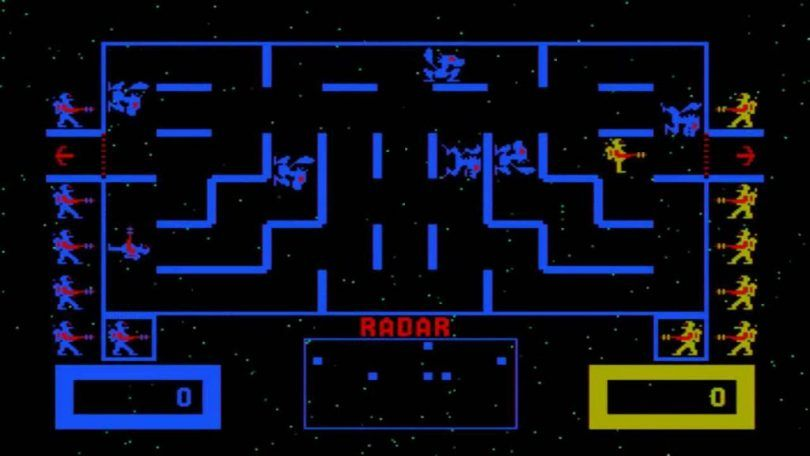
\includegraphics[scale=0.4]{assets/lateximg/WizardOfWor}\\
  Image Source: \texttt{https://www.moregameslike.com/}
  \section{Introduction}

  This report is a report for the development of a clone of the 80's Arcade game \textbf{Wizard Of Wor}. The game said game, which this project is a clone of is an arcade game developed by Midway. This report will start by introducing the reader to the original Game, identifying the gameplay mechanics of the game, and other important key-features of this game.

  We will than go on and identifying the possible problems to be solved when creating a game like Wizard Of Wor and the solutions for these. In the same section, we will also discuss the viability of implementing all the possible features of this game. Since the there are many features in the said game, some of the features that are present in the original game will be omitted. This will be discussed here.

  The report will than go on to discuss the design the development process of the game, as well as challenges that surfaced during development. Additionally, this section will discuss the decision made regard the design and implementation of the features of the game.

  In the next section, the report will showcase, and discuss the results of the project. What could be done differently, future plans, and other discussions related to the project.

  \subsection{Project structure and Libraries}
  The whole project is written in the language C++, which is a common language found within the area of Game development. The language itself is notable for it's low-level nature and being very close to hardware level, thus it is also by implication very high performing programming language.

  Addtionally, the project will use SDL, which is a library that is very commonly used within game development. According to Wikipedia, SDL is a library that provides an hardware abstraction layer for computer multimedia hardware components. In other words, the library is similar to OpenGL, but provides more functionallities than OpenGL, which is a library used for computer graphics. Examples of titles that are developed using SDL are \textbf{Brütal Legend}, \textbf{Memoria}, and \textbf{Robin Hood}.

  \section{Background and Specification}
  This section will break down the original game, and from it identify the key-features and specifications for it, thus also for this project as a whole.

  \begin{figure}
    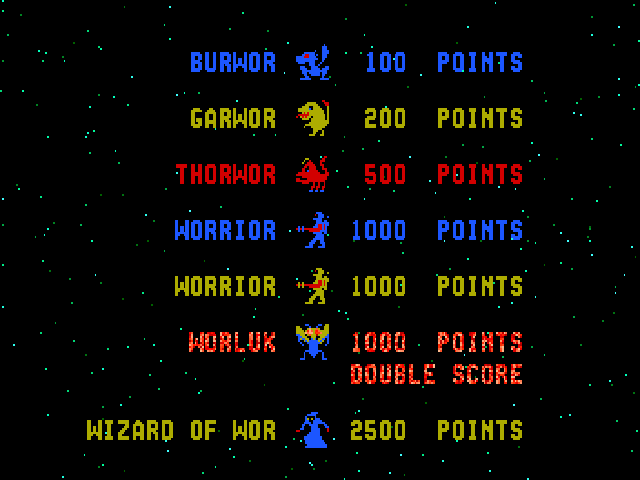
\includegraphics[scale=0.7]{assets/lateximg/Monstertable}
    \caption{The Table of the monsters in the game, including the both players (the Worriors). Source: \texttt{https://extralives.files.wordpress.com}}
    \label{monstertable}
  \end{figure}

  \subsection{The Original Game}

  The original game is playable by up to two people. The players, also known as \textbf{Worriors} in the game, are running around in a two dimensional maze with a lot of Monsters. The objective is to gather as much score as possible. Score points is acquired by killing the monsters in the Maze. When a maze is cleared, they move on two the next level, which is another maze filled with monsters. The end score is the collective points collected from the process of killing monster and clearing as many levels as possible. Each maze has it's own difficulties in the form of how design, and amount of monsters.

  In the case that two players are playing the game. The players can also gather points by killing each other.

  The players loses lives if they are killed by the monsters. From the beginning, each player starts with 3 lives. Monsters can kill the player by firing on them and by walking into the player. Hence, the player will die if he/she collides with a monster.

  There are 5 different typse of monsters in this game, each worth different amounts of points and have different attributes to them. These can be found in the picture figure \ref{monstertable}.

  A more detailed explanation of the monsters:
  \begin{itemize}
    \item \textbf{The Burwor}: The easiest monster to kill, no special features, and moves a little bit slower than the players.
    \item \textbf{The Garwor}: A monster that is similar to the Burwor, but can become invisible.
    \item \textbf{The Thorwor}: This monster is faster than the Burwor and the Garwor. It is also capable of going invisible.
    \item \textbf{The Worluk}: This monster will not attack the players, instead, it will try to escape the maze. The player will still pass the level if this monster escaped, but killing the monster will give the player double points in the next level. Note that this monster moves very fast
    \item \textbf{The Wizard of Wor}: This monster is kind of main boss, though it is still killed with one shot, it moves faster than all the other monsters except for the Worluk. It is also capable of teleportation. Not that the game is named after this monster.
  \end{itemize}

  In addition, as mentioned in the introduction, the Worriors, i.e. the player can also kill eachother, with a profit of 1000 points each kill, the tradeoff in doing so is that the killing of the other monster will be harder. However, note that killing the other player awards more points than at least 3 of the monsters. Thus a very interesting situation of two players \textbf{Prisoners Dilemma} arises in this game(See appendix).

  Other interesting features of this game is the use of voice synthetisation in form of tauntings performed by the Wizard of Wor himself.

  \subsection{Key features and project specifications}
  From the previous subsection following key features can be found:
  \begin{itemize}
    \item Two Players Control.
    \item The Maze - Each level is a different maze. This also includes the movemente in the maze.
    \item AI - Each monster moves on it's own according to an AI, making this game a multiagent system with many different agents. Note that there are 5 unique types of monsters in this game, thus around 5 different kind of AI's in the game.
    \item Collision detection with the projectiles, and the monsters.
    \item Sound- and voice synthetisation for the sound samples and the tauntings by the wizard.
    \item Other aesthetics such as animations, and different sprites.
  \end{itemize}
  This project will try to implement as many key-features as possible, but focuses mainly on the first four. This is beacuse the last 2 are mainly for aesthetics of the game, thus not a key mechanics for the game itself. These will be implemented if time allows it to.

  \subsection{Problems present}
  There are different kind of problems to be solved, if one ought to make a clone of Wizard Of Wor. This subsection will take the problems related to the key-features as identified in the last subsection.

  First of, the whole two players game notion is a problem by itself. Not only does it relate to the main mechanics of the game. It also relates a lot to the user experience from the players playing this game. Finding a good set of controlls can be identified as a challenge in the making of this game.

  Moving on to the maze, One of the main problems that the maze introduces to the game is the movement, and bounding each entity inside the maze. There are various ways of representing the maze internally in the game, thus finding the optimal model for the maze is a problem by itself. This problem also relates to the player controll stated in the last paragraph. It also influences the modelling of the AI for the monsters.

  As already stated above, collision detection is needed in this game. There are two kinds of collision to detect. The Players and monsters against a projectile, and the collision monster against player.

  The AI is probably one of the most complex of these problems, This can be broken down into two types of problems: Path finding and Heuristics. There are many algorithms for path searching, including depth first, and breadth first search. There are greedy approaches and algorithms related to dynamic programming. Heuristics problems are related to the path findings, since using good heuristics can greatly influence the performance in time complexity of the path searching algorithm. Heuristics are also good for differentiate each of the unique AI controlled entities behaviour pattern. In this game, due to the existence of reload time, a Heuristics for when to shoot a projectile is important.

  \section{Implementation}
  This section will give a short description of the development process outlining the design, and modelling choices made, as well as the challenges that came up related to the development of this game. In the beginning of the project, we were given a set of C++ code as a starting point. In this library Basic implementation of a gameloop, a basic set of classes representing the game objects, and each objects components, a basic implementation of a player, and a set of classes that provides functionalities like rendering of sprites and basic IO handling. In addition, a basic implementation of collision detection, and collision handling are implemented.

  \section{Two Players Controll}
  This was more of a design problem rather than an implementation problems.
  \section{Results and Discussion}

  \section{Appendix}
  \subsection{Prisoners Dilemma}

  In the area of Game Theory, the prisoners dilemma is a two players game that can be formulated as following:

  Two people have commited a crime and are in for interogation, they are also facing a sentence of one year in prison. The interogator presents the two parties with a choice to tell on he's or her's partner for 0 years in prison. The partner in crime will be facing a sentence of 5 years. But if both parties tell on each other, they both will face a sentence on 3 years.

  Given these choices of possible outcome. One can quickly infer that the better move in one round of the game for an individual player is to back talk on your partner and betray them. However note that, in if neither betray each other, both faces a collective minimal punishment.

  This is interesting for Wizard Of Wor, since both players are faced with either shooting the monsters in the maze, or shoot the other player for more points. Note that though, betraying eachother has a consequence in Wizard of Wor, the players will have a harder time killing the monsters if they are busy killing each other, and if one of them has depleted their lives.
\end{document}